\chapter{Reinforcement Learning}
\label{ch:rl_grundlagen}

Dieses Kapitel legt die theoretischen Grundlagen für die in dieser Arbeit entwickelte Lösung. Es führt in das Paradigma des Reinforcement Learning (\ac{RL}) ein und erläutert die mathematische Formalisierung von Entscheidungsproblemen als Markov-Entscheidungsprozesse. Ein tieferes Verständnis dieser Konzepte – insbesondere der Funktionsweise von Policy-Gradient-Methoden und der Proximal Policy Optimization (PPO) – ist essenziell, um die in Kapitel \ref{ch:ppo_bedingt} vorgestellten algorithmischen Anpassungen (Gradient Gating) für gemischte Aktionsräume nachvollziehen zu können.

\section{Einführung in Reinforcement Learning}

Reinforcement Learning (\ac{RL}) ist ein Teilgebiet des maschinellen Lernens, das sich besonders für komplexe sequentielle Entscheidungsprobleme eignet, bei denen ein explizites Lehren des korrekten Verhaltens ("Supervised Learning") aufgrund der Vielschichtigkeit der Aufgabe schwierig ist. Da in der vorliegenden Arbeit eine Steuerung für ein dynamisches System automatisiert werden soll, bietet \ac{RL} den passenden methodischen Rahmen. Eines der Standardwerke \cite{sutton2018rl} definiert \ac{RL} wie folgt: 
\\

\textit{"Beim verstärkenden Lernen geht es darum, zu lernen, was zu tun ist – wie Situationen auf Handlungen abgebildet werden können –, um
ein numerisches Belohnungssignal zu maximieren. Dem Lernenden wird nicht gesagt, welche Handlungen er ausführen soll,
sondern er muss durch Ausprobieren herausfinden, welche Handlungen die größte Belohnung bringen."}
\\

Im \ac{RL} werden also Agenten bzw. Policies durch Interaktion mit ihrer Umgebung trainiert, um eine maximale kumulative Belohnung zu erzielen.
Dies unterscheidet \ac{RL} von überwachten Lernverfahren, bei denen Modelle anhand von gekennzeichneten Beispieldaten trainiert werden \cite[Kap. 1]{sutton2018rl}.
Um einen \ac{RL}\hyp{}Agenten zu trainieren, muss eine Umgebung definiert werden, in der der Agent Erfahrungen sammeln kann \cite{gymnasium_basic_usage}.


\section{Markov\hyp{}Entscheidungsprozesse}
Um ein reales Problem für einen \ac{RL}\hyp{}Algorithmus zugänglich zu machen, muss es zunächst formalisiert werden. Das Konzept des \ac{MDP} liefert hierfür das mathematische Fundament. Es modelliert Entscheidungsprobleme, bei denen ein Agent in einer Umgebung agiert, um eine maximale Belohnung zu erzielen \cite[Kap. 3]{sutton2018rl}. Die korrekte Definition des MDPs ist daher der erste und wichtigste Schritt, um die reale Aufgabenstellung in eine durch den Computer lösbare Form zu überführen.
Ein \ac{MDP} wird durch das folgende 4\hyp{}Tupel definiert:
\\

\((S, A, P, R)\)
\\

wobei:
\begin{itemize}
    \item \textbf{S}: Eine endliche Menge von Zuständen, die die möglichen Situationen in der Umgebung rep®räsentieren.
    \item \textbf{A}: Eine endliche Menge von Aktionen, die der Agent ausführen kann.
    \item \textbf{P}: Die Übergangswahrscheinlichkeitsfunktion, die angibt, mit welcher Wahrscheinlichkeit der Agent von einem Zustand zu einem anderen Zustand übergeht,
    wenn er eine bestimmte Aktion ausführt. Formal ausgedrückt als \(P(s'|s,a)\), wobei \(s\) der aktuelle Zustand, \(a\) die Aktion und \(s'\) der Folgezustand ist \cite[Kap. 3.1]{sutton2018rl}.
    \item \textbf{R}: Die Belohnungsfunktion, die angibt, welche Belohnung der Agent erhält, wenn er eine bestimmte Aktion in einem bestimmten Zustand ausführt.
\end{itemize}

\label{sc:agent_environment_interaction}

\begin{figure}[h]
    \centering
    \includegraphics[width=0.6\textwidth]{chapters/bilder/Agent_Env_Interaktion.png}
    \caption{Interaktion zwischen Agent und Umgebung im Reinforcement Learning (Quelle: \cite[Kap. 3.1]{sutton2018rl})}
    \label{fig:rl_agent_environment}
\end{figure}

Bei jedem Zeitschritt \(t\) befindet sich der Agent in einem Zustand \(s_t \in S\), wählt eine Aktion \(a_t \in A\) basierend auf seiner Policy\footnote{Eine Policy beschreibt das Verhalten des Agenten. Sie ordnet jedem Zustand eine Aktion bzw. eine Wahrscheinlichkeitsverteilung über mögliche Aktionen zu.} \(\pi\) aus,
führt die Aktion aus und erhält eine Belohnung \(r_t = R(s_t, a_t)\). Die Umgebung wechselt dann in einen neuen Zustand \(s_{t+1}\) basierend auf der Übergangswahrscheinlichkeit \(P(s_{t+1}|s_t, a_t)\).
Der Prozess wiederholt sich solange, bis ein Abbruchkriterium erreicht ist (z.B. eine maximale Anzahl von Schritten oder das Erreichen eines Zielzustands).
Beim Durchlaufen eines \ac{MDP} entsteht eine Folge von Zuständen, Aktionen und Belohnungen, die als \textbf{Trajektorie} bezeichnet wird \cite[Kap. 3.1]{sutton2018rl}:
\\

\((s_0, a_0, r_0, s_1, a_1, r_1, s_2, a_2, r_2, ...)\)
\\  

Diese Trajektorie repräsentiert die Erfahrung des Agenten in der Umgebung und wird verwendet, um die Policy zu verbessern und den Agenten zu trainieren.
\\


\section{Differenzierung verschiedener Aktionsraumklassen}
\label{sc:Aktionsraumklassen}
Die Beschaffenheit des Aktionsraums ist ein wesentliches Merkmal jedes \ac{RL}\hyp{}Problems, da sie bestimmt, welche Handlungen dem Agenten zur Verfügung stehen. Eine präzise Unterscheidung ist hierbei notwendig, da unterschiedliche Raumklassen fundamental unterschiedliche Anforderungen an die Netzwerkarchitektur und den Lernalgorithmus stellen.
Obwohl in der Literatur diverse Modellierungen existieren, beschränkt sich die folgende Betrachtung auf die drei für diese Arbeit relevanten Kategorien:
\begin{itemize}
    \item \textbf{Diskrete Aktionsräume:}
    In einem diskreten Aktionsraum wählt der Agent aus einer begrenzten Anzahl vordefinierter Optionen.
    Ein anschauliches Beispiel ist ein herkömmlicher Lichtschalter: Es gibt nur die zwei Zustände \textit{Ein} und \textit{Aus}. Zwischenstufen sind nicht möglich.
    \item \textbf{Kontinuierliche Aktionsräume:}
    Hier werden Aktionen durch Werte innerhalb eines bestimmten Bereichs dargestellt, was theoretisch unendlich viele Abstufungen erlaubt.
    Vergleichbar ist dies mit einem Dimmer für Licht, bei dem die Helligkeit nicht nur an- oder ausgeschaltet, sondern stufenlos (z.\,B. auf $75\,\%$) geregelt werden kann. In der Praxis entspricht dies oft Steuergrößen wie Lenkwinkeln oder Motorkraft.
    \item \textbf{Hybride Aktionsräume:}
    Viele reale Probleme erfordern eine Mischung aus beiden Typen. Hybride Räume bestehen sowohl aus diskreten als auch aus kontinuierlichen Komponenten.
    Dies lässt sich am Beispiel eines Autos mit Schaltgetriebe verdeutlichen: Das Einlegen eines Gangs ist eine diskrete Entscheidung (z.\,B. 1., 2. Gang), während das Gasgeben und Lenken kontinuierliche Eingaben sind.
\end{itemize}

Diese Arbeit konzentriert sich speziell auf eine Kombination zweier Konzepte: hybride und bedingte Aktionsräume. Während der hybride Aspekt die Mischung aus diskreten und kontinuierlichen Aktionen beschreibt, führt der bedingte Charakter hierarchische Abhängigkeiten ein. Das bedeutet, die Auswahl einer übergeordneten diskreten Aktion bestimmt, welche untergeordneten Aktionen (oft kontinuierlich) zur Verfügung stehen. In der Literatur werden solche Strukturen auch als parametrisierte Aktionsräume bezeichnet. Ansätze wie sie in \cite{bamford2021generalising} vorgestellt werden, nutzen eine explizite Baumstruktur, um diese Abhängigkeiten im Kontext von Echtzeit-Strategiespielen (RTS) zu modellieren um eine Reduktion der Modellkomplexität zu erreichen. Die vorliegende Arbeit überträgt diesen Grundgedanken auf den Luftverkehrskontext. Um die kausalen Abhängigkeiten während des Trainings zu wahren, wird im weiteren Verlauf die Methode des \textit{Gradient Maskings} eingesetzt.

\subsection{Extraktion von Aktionen aus neuronalen Netzen}
\label{sc:action_extraction}
Die Wahl der Aktionsraumklasse hat direkte Auswirkungen auf die Architektur der Ausgabeschicht (Output Layer) des neuronalen Netzes und die Art und Weise, wie Aktionen aus den Netzwerkausgaben abgeleitet werden.

\subsubsection*{Diskrete Aktionsräume}
Stable Baselines3 \cite{sb3} modelliert diskrete Aktionsräume mittels einer kategorialen Verteilung (Categorical Distribution). Hierbei besitzt die Ausgabeschicht des Netzwerks für jede mögliche diskrete Aktion genau ein Neuron. Die Aktivierungswerte dieser Neuronen (Logits) werden durch eine \emph{Softmax}-Funktion in Wahrscheinlichkeiten umgewandelt, wobei die Summe aller Wahrscheinlichkeiten $1$ ergibt.
\vspace{\baselineskip}

Während des Trainings wird eine Aktion stochastisch basierend auf diesen Wahrscheinlichkeiten gesamplet. Ein wesentlicher Nachteil diskreter Aktionsräume liegt im sogenannten \emph{Fluch der Dimensionalität} bei feingranularen Steuerungsaufgaben. Soll eine kontinuierliche Größe (z.\,B. ein Lenkwinkel) präzise gesteuert werden, muss der Wertebereich diskretisiert werden. Eine Erhöhung der Präzision erfordert eine feinere Diskretisierung, was zu einem linearen Anstieg der benötigten Ausgangsneuronen führt. Soll beispielsweise ein Bereich von $-180^\circ$ bis $+180^\circ$ in $1^\circ$-Schritten abgebildet werden, benötigt das Netzwerk bereits $361$ Ausgangsneuronen. Bei mehrdimensionalen Aktionsräumen (z.\,B. Lenken und Beschleunigen) wächst die Anzahl der benötigten Kombinationen exponentiell an (kartesisches Produkt der Einzelaktionen), was das Training ineffizient macht \cite{lillicrap2015continuous}.

\subsubsection*{Kontinuierliche Aktionsräume}
Analog zu den diskreten Räumen modelliert Stable Baselines3 \cite{sb3} kontinuierliche Aktionsräume durch die Parametrisierung einer Wahrscheinlichkeitsdichtefunktion, standardmäßig einer Gauß-Verteilung (Normalverteilung). Anstatt Wahrscheinlichkeiten für diskrete Werte auszugeben, liefert das Netzwerk die Parameter der Verteilung, typischerweise den Erwartungswert $\mu$ (Mean) und die Standardabweichung $\sigma$ (Standard Deviation).
Für einen $n$-dimensionalen kontinuierlichen Aktionsvektor benötigt das Netzwerk somit lediglich $2n$ Ausgangsneuronen.

\section{Differenzierung verschiedener RL\hyp{}Algorithmen}

Nach der Formalisierung des Problems als MDP stellt sich die Frage nach dem geeigneten Lösungsverfahren. Die Wahl des Algorithmus ist dabei maßgeblich von den Eigenschaften des Problems, wie der Beschaffenheit des Zustands- und Aktionsraums, abhängig.
Algorithmen des \ac{RL} lassen sich grundlegend in modellbasierte und modellfreie Ansätze unterteilen \cite[Kap. 8]{sutton2018rl}. 
Während modellbasierte Verfahren ein internes Abbild der Systemdynamik (\textit{Transition Model}) erlernen, 
operieren modellfreie Algorithmen ausschließlich auf Basis der durch Interaktion gesammelten Erfahrungen. Da die Modellierung 
komplexer Umgebungen wie der Flugverkehrssteuerung oft mit hohen Unsicherheiten behaftet ist, fokussiert sich diese Arbeit auf modellfreie Ansätze.
\vspace{\baselineskip}

Innerhalb der modellfreien Algorithmen wird primär zwischen wertbasierten Methoden (z.\,B. Q\hyp{}Learning) und \textit{Policy\hyp{}Gradient}\hyp{}Methoden unterschieden. 
Die Wahl fällt in dieser Arbeit auf Letztere, da \textit{Policy\hyp{}Gradient}\hyp{}Methoden inhärent besser für kontinuierliche oder hochdimensionale Aktionsräume 
geeignet sind und eine direktere Optimierung des angestrebten Verhaltens erlauben \cite[Kap. 13.2]{sutton2018rl}.

\subsection{Policy\hyp{}Gradient\hyp{}Methoden}
Da die zu lösende Steuerungsaufgabe einen kontinuierlichen und hochdimensionalen Aktionsraum aufspannt, bieten sich Policy\hyp{}Gradient\hyp{}Methoden als Lösungsansatz an.
Im Gegensatz zu wertbasierten Ansätzen, die zunächst eine Wertfunktion lernen und daraus eine Politik ableiten, optimieren \textit{Policy\hyp{}Gradient}\hyp{}Methoden die Strategie $\pi_\theta$ des Agenten unmittelbar. 
Die Policy wird dabei als differenzierbares, parametrisiertes Modell — in der Regel ein künstliches neuronales Netzwerk — aufgefasst, 
das für einen gegebenen Zustand $s$ eine Wahrscheinlichkeitsverteilung über das Aktionsspektrum ausgibt.
\vspace{\baselineskip}

Das Ziel der Optimierung ist die Maximierung der erwarteten kumulativen Belohnung $J(\theta)$. Die Anpassung der Parameter $\theta$ erfolgt durch den 
Aufstieg entlang des Gradienten $\nabla_\theta J(\theta)$, wodurch die Eintrittswahrscheinlichkeit von Aktionen, die zu überdurchschnittlichen Erträgen 
führen, systematisch erhöht wird \cite[Kap. 13.2]{sutton2018rl}.
\vspace{\baselineskip}

Die folgende Tabelle \ref{tab:ppo_vars} fasst die mathematischen Symbole und deren spezifische Bedeutung zusammen, die im Kontext von Policy-Gradient-Methoden und insbesondere \ac{PPO} relevant sind. Diese Variablen bilden die Grundlage für die formale Beschreibung der Lernalgorithmen und deren Anpassungen, die in den folgenden Kapiteln behandelt werden.

\begin{table}[H]
\centering
\begin{tabular}{|p{2cm}|p{3cm}|p{7cm}|} 
\hline
\textbf{Variable} & \textbf{Bedeutung} & \textbf{Rolle im PPO\hyp{}Algorithmus} \\
\hline
$\theta$          & Policy\hyp{}Parameter & Der Vektor der trainierbaren Gewichte des neuronalen Netzwerks (Actor). \\
$\pi_\theta$      & Policy & Liefert Wahrscheinlichkeiten über Aktionen; Parameter $\theta$ werden trainiert \\
$V_\phi$          & Wertfunktion (Critic) & Schätzt erwarteten kumulierten Reward ab einem Zustand; Parameter $\phi$ werden trainiert \\
$J(\theta)$       & Performance Objective & Die Zielfunktion (erwarteter kumulierter Return), die maximiert werden soll \\
$R_t$             & Return & Diskontierte Summe der Rewards ab Zeit $t$ \\
$\gamma$          & Dis\-kont\-ie\-rungs\-faktor & Bestimmt die Gewichtung zukünftiger Belohnungen im Return $R_t$ \\
$A_t$             & Advantage & Vorteil einer Aktion gegenüber dem Durchschnitt: $A_t = R_t - V_\phi(s_t)$ \\
$\pi_{\text{old}}$ & Alte Policy & Policy, die während des Rollouts verwendet wurde; dient zur Berechnung des Probability Ratio \\
$r_t(\theta)$       & Probability Ratio & Verhältnis zwischen aktueller und alter Policy: $\frac{\pi_\theta(a_t|s_t)}{\pi_{\text{old}}(a_t|s_t)}$ \\
$L^{\text{CLIP}}(\theta)$ & Clipped Surrogate Objective & Maximiert den erwarteten Vorteil, begrenzt durch Clipping, um große Policy\hyp{}Updates zu vermeiden \\
$L_t^{VF}(\phi)$  & Value Function Loss & Der quadratische Fehler (MSE) zwischen der Schätzung des Critics $V_\phi$ und dem realisierten Return $R_t$. \\
$S[\pi_\theta]$   & Entropie\hyp{}Bonus & Ein Maß für die Unvorhersehbarkeit der Policy; verhindert eine zu frühe Konvergenz auf ein lokales Optimum. \\
$L_t^{total}$     & Totale Verlustfunktion & Die gewichtete Kombination aller Verlustkomponenten, die vom Optimierer minimiert wird ($\approx -J$). \\
$c_1, c_2$        & Ge\-wich\-tungs\-ko\-ef\-fi\-zi\-en\-ten & Steuern den Einfluss von Value Loss und Entropie auf die kombinierte Verlustfunktion \\
$\epsilon$         & Clipping\hyp{}Parameter & Bestimmt die Grenze für das Clipping im Surrogate Objective \\
$n\_epochs$       & Anzahl der Trainings\hyp{}Epochen & Gibt an, wie oft die Policy und Wertfunktion pro Rollout aktualisiert werden \\
\hline
\end{tabular}

\caption{Übersicht der wichtigsten Variablen im PPO\hyp{}Algorithmus}
\label{tab:ppo_vars}
\end{table}

\subsection{Actor\hyp{}Critic\hyp{}Architektur}
Um die Varianz der Gradientenschätzung zu reduzieren und den Lernprozess zu stabilisieren, greift diese Arbeit auf eine weit verbreitete Erweiterung der reinen Policy\hyp{}Gradient\hyp{}Methoden zurück: die \textit{Actor\hyp{}Critic}\hyp{}Architektur.
Diese kombiniert die Vorteile von Policy\hyp{}Methoden mit wertbasierten Ansätzen \cite[Kap. 13.5]{sutton2018rl}:
\begin{itemize}
    \item Der \textbf{Actor} (die Policy) ist für die Auswahl der Aktionen verantwortlich.
    \item Der \textbf{Critic} (die Wertfunktion $V_\phi$) schätzt den Erwartungswert der zukünftigen Belohnungen ab einem Zustand.
\end{itemize}
Durch die Gegenüberstellung der tatsächlichen Erträge mit der Schätzung des Critics lässt sich der sogenannte \textbf{Advantage} $A_t$ berechnen.
Dieser gibt an, um wie viel besser eine gewählte Aktion im Vergleich zum Durchschnitt aller möglichen Aktionen in diesem Zustand war. Der Advantage
dient als rauscharmes Signal für das Update des Actors und reduziert die Varianz des Gradienten signifikant \cite[Kap. 13.5]{sutton2018rl}.

\section{Proximal Policy Optimization}
Als konkreter Algorithmus kommt in dieser Arbeit die \ac{PPO} zum Einsatz. Sie stellt eine Weiterentwicklung innerhalb der \textit{Policy\hyp{}Optimization}\hyp{}Verfahren dar \cite{OriginalPPO} und gilt derzeit als State-of-the-Art für viele kontinuierliche Kontrollprobleme, da sie eine gute Balance zwischen Benutzerfreundlichkeit, Stabilität und Effizienz bietet.
\ac{PPO} setzt auf eine Actor\hyp{}Critic\hyp{}Architektur und adressiert die Instabilität klassischer Gradientenverfahren, bei denen zu große Aktualisierungsschritte die Policy in Regionen des Parameterraums treiben können, aus denen eine Erholung kaum möglich ist.
\vspace{\baselineskip}

Der Kern von PPO ist das \textit{Clipped Surrogate Objective}. Durch diese Zielfunktion wird die Änderung der Policy pro Update\hyp{}Schritt begrenzt (Clipping).
PPO bietet gegenüber verwandten Methoden wie TRPO (\textit{Trust Region Policy Optimization}) eine höhre Hyperparameterstabilität \cite[Abschn. 2.2]{OriginalPPO} und reduziert somit die Anfälligkeit gegenüber schlechten Hyperparametereinstellungen.
\vspace{\baselineskip}

Die Wahl von PPO für die Flugverkehrssteuerung begründet sich durch seine Robustheit gegenüber Hyperparametereinstellungen und die effiziente Handhabung
diskret\hyp{}kontinuierlicher Aktionsräume. Zudem erlaubt die Implementierung in \textit{Stable Baselines3} \cite{sb3} eine modulare Anpassung der Netzwerkarchitektur,
was für das in dieser Arbeit vorgestellte \textit{Gradient Masking} essentiell ist.

\subsection{Trainingsablauf}
Für die spätere Implementierung des \textit{Gradient Gating} ist das Verständnis des iterativen Trainingsprozesses essenziell. Es ist entscheidend nachzuvollziehen, wo konkret Gradienten entstehen und an welcher Stelle diese verarbeitet werden.
Der PPO\hyp{}Algorithmus operiert dabei in zwei Hauptphasen: der \textbf{Rollout\hyp{}Phase} und der \textbf{Optimierungsphase}. In der Rollout\hyp{}Phase interagiert der Agent
mit der Umgebung, sammelt Trajektorien (siehe \ref{sc:agent_environment_interaction}). 
Diese Daten werden in einem sogenannten \textit{Rollout\hyp{}Buffer} gespeichert.
In der Optimierungsphase wird die Policy anhand der gesammelten Daten aktualisiert. Hierbei wird das \textit{Clipped Surrogate Objective} verwendet,
um die Policy\hyp{}Parameter $\theta$ so anzupassen, dass die erwartete kumulative Belohnung maximiert wird, ohne dabei zu große Änderungen an der Policy vorzunehmen.

\begin{algorithm}[H]
\begin{algorithmic}[1]
\State Initialisiere Policy $\pi_\theta$ und Value Function $V_\phi$
\State Initialisiere Umgebung
\While{nicht fertig}
    \State Reset Umgebung
    \While{Episode nicht beendet}
        \State Beobachte aktuellen Zustand $s_t$
        \State Berechne Aktionsverteilung $p = \pi_\theta(s_t)$
        \State Wähle Aktion $a_t$ stochastisch aus $p$
        \State Führe Aktion $a_t$ aus
        \State Beobachte Belohnung $r_t$ und neuen Zustand $s_{t+1}$
        \State Speichere $(s_t, a_t, r_t, \log p(a_t))$
        \State $t \gets t+1$
    \EndWhile
    \State Alle Rewards aufsummieren und mit $\gamma$ gewichten
    \State Alle Advantages berechnen
    \State Alte Policy speichern
    \For{$epoch = 1 \dots n\_epochs$}
        \State Generiere Minibatches aus den gesammelten Trajektorien
        \For{jedes $minibatch$}
            \State Berechne Logarithmische Wahrscheinlichkeit und Entropie
            \State Berechne Probability Ratio ($r_t(\theta)$)
            \State Berechne Clipped Surrogate Objective ($L^{\text{CLIP}}(\theta)$)
            \State Berechne Critic Loss ($L_t^{VF}(\phi)$)
            \State Berechne Entropie-Bonus ($S[\pi_\theta]$)
            \State Gewichte der Policy ($\pi_\theta$) \& Value Function ($V_\phi$) aktualisieren
        \EndFor
    \EndFor
\EndWhile
\end{algorithmic}
\caption{Beispielhaft vereinfachter PPO-Trainingsablauf}
\label{alg:ppo_training}
\end{algorithm}


Der in Algorithmus \ref{alg:ppo_training} dargestellte Ablauf verdeutlicht die Trennung zwischen Datenerhebung und Optimierung. 
Während der Rollout\hyp{}Phase (Zeilen 3--13) wird die \textit{logarithmische Wahrscheinlichkeit} der gewählten Aktionen direkt im Buffer gespeichert. 
Dies ist essenziell, da diese Werte im späteren Verlauf als Referenz für die \textit{Alte Policy} ($\pi_{\text{old}}$) dienen.
\vspace{\baselineskip}

In der Optimierungsphase (Zeilen 14--27) findet die eigentliche Anpassung der Netzwerkgewichte statt. Hierbei werden die im Vorfeld berechneten 
Advantage\hyp{}Werte genutzt, um das \textit{Clipped Surrogate Objective} zu berechnen. In dieser Arbeit wird der Fokus im Abschnitt \ref{sc:ppo_anpassung}
auf diese Phase gelegt, da hier das \textit{Gradient Masking} implementiert wird.

\subsection{Die kombinierte Verlustfunktion}
Ein zentraler Bestandteil der Optimierungsphase ist die Verlustfunktion. Sie stellt zugleich den entscheidenden Eingriffspunkt für das in Kapitel \ref{ch:ppo_bedingt} vorgestellte \textit{Gradient Masking} dar, weshalb eine detaillierte Aufschlüsselung ihrer Komponenten für das Verständnis der späteren Modifikationen unerlässlich ist.
In der praktischen Implementierung von \ac{PPO} werden die Parameter des Actors ($\theta$) und des Critics ($\phi$) simultan über eine solche kombinierte Funktion optimiert. Da Frameworks wie PyTorch auf die Minimierung einer Zielfunktion ausgelegt sind, wird das Maximierungsproblem des Actors durch Negation in ein Minimierungsproblem überführt. Die totale Verlustfunktion ergibt sich als gewichtete Summe \cite[Glg. 9]{OriginalPPO}:

\begin{equation}
    L_t^{total}(\theta, \phi) = \hat{\mathbb{E}}_t \left[ -L_t^{CLIP}(\theta) + c_1 L_t^{VF}(\phi) - c_2 S[\pi_\theta](s_t) \right]
\end{equation}

Dabei setzen sich die Komponenten wie folgt zusammen:

\begin{itemize}
    \item \textbf{Actor\hyp{}Loss} ($-L_t^{CLIP}$): Das \textit{Clipped Surrogate Objective} begrenzt die Änderung der Policy \cite[Abschn. 3]{OriginalPPO}. Da \ac{PPO} den Vorteil $A_t$ maximieren möchte, wird dieser Term für den Gradientenabstieg negiert:
    \begin{equation}
        L_t^{CLIP}(\theta) = \min \big( r_t(\theta) A_t, \text{clip}(r_t(\theta), 1-\epsilon, 1+\epsilon) A_t \big)
        \label{eq:clip_loss}
    \end{equation}
    
    \item \textbf{Critic\hyp{}Loss} ($L_t^{VF}$): Der \textit{Value Function Loss} beschreibt den quadratischen Fehler zwischen der Vorhersage des Critics und dem tatsächlichen Return $R_t$:
    \begin{equation}
        L_t^{VF}(\phi) = (V_\phi(s_t) - R_t)^2
        \label{eq:value_loss}
    \end{equation}
    Dieser Term wird addiert, da er direkt minimiert werden soll.

    \item \textbf{Entropie\hyp{}Bonus} ($S[\pi_\theta]$): Dieser Term misst die Unvorhersehbarkeit der Policy. Er wird subtrahiert, um die Entropie zu maximieren und somit vorzeitige Konvergenz gegen lokale Optima zu verhindern. Dieser Bonus fördert die Exploration, indem er die Policy dazu anregt, eine diversifizierte Aktionsverteilung beizubehalten. Exploration vs. Exploitation ist ein zentrales Thema im \ac{RL}, da der Agent sowohl neue Strategien ausprobieren (Exploration) als auch bewährte Strategien nutzen (Exploitation) muss, um langfristig optimale Ergebnisse zu erzielen \cite[Kap. 2]{sutton2018rl} \cite[Abschn. 5]{OriginalPPO}.
\end{itemize}

Der Zusammenhang zwischen diesen Komponenten ist essentiell für die Stabilität: Ein präziser Critic minimiert $L_t^{VF}$, was zu verlässlichen Advantage\hyp{}Schätzungen $A_t$ führt. Diese bilden wiederum die Grundlage für zielgerichtete Updates des Actors über $L_t^{CLIP}$. Die Hyperparameter $c_1$ und $c_2$ steuern dabei die Gewichtung zwischen Genauigkeit der Wertfunktion, Optimierung der Policy und dem Erhalt der Explorationsfähigkeit.

\subsection{Gradientenbasierte Optimierung}
Die Minimierung der zuvor beschriebenen Verlustfunktion erfolgt technisch durch Gradientenabstieg. Ein Verständnis dieser Mechanismen ist entscheidend, um nachzuvollziehen, wie durch gezieltes Gating bestimmte Parameter situationsbedingt vom Training ausgeschlossen werden können.

\begin{figure}[htbp]
    \centering
    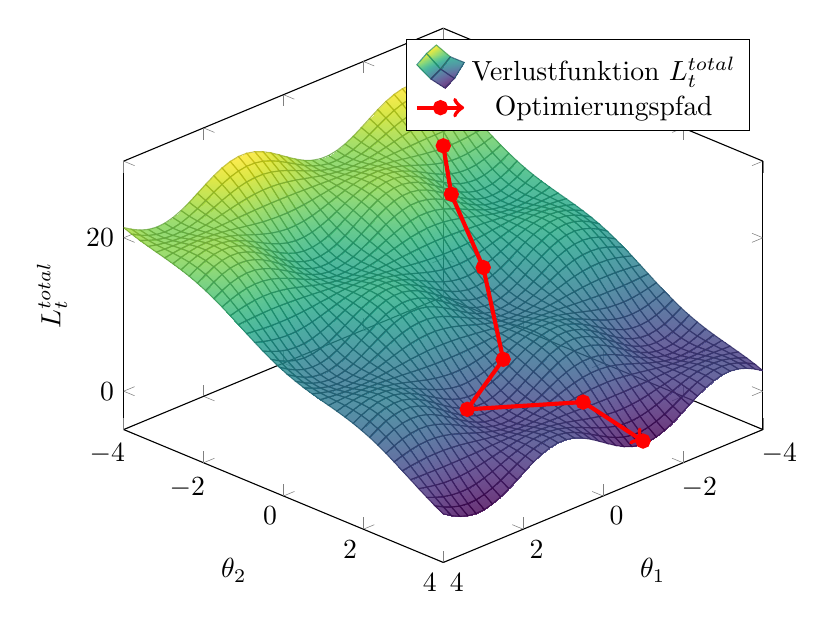
\begin{tikzpicture}
        \begin{axis}[
            width=0.8\textwidth,
            view={135}{35}, % Blickwinkel angepasst für Diagonale
            xlabel=$\theta_1$,
            ylabel=$\theta_2$,
            zlabel=$L_t^{total}$,
            colormap/viridis,
            zmin=-5, zmax=30, % Angepasste Z-Grenzen
        ]
        
        % 1. Die Oberfläche: Eine geneigte Ebene mit Wellen (lokale Minima/Maxima)
        % Wirkt komplexer ("non-convex") und fällt Richtung (4,4) ab.
        \addplot3[
            surf,
            shader=faceted interp,
            domain=-4:4,
            y domain=-4:4,
            samples=40, % Mehr Samples für die Wellen
            opacity=0.8
        ] {12 - 2.5*y + 2.5*sin(deg(x*1.5))*cos(deg(y*1.5))};

        % 2. Der Pfad des Gradientenabstiegs
        % Startet "oben" (bei ca. -3, -3) und driftet durch Rauschen stärker in x-Richtung ab
        \addplot3[
            color=red,
            mark=*,
            mark size=2pt,
            line width=1.5pt,
            ->
        ] coordinates {
            (-3, -3, 19.0)     % Start
            (-2.2, -2.0, 16.6) % Starker Drift nach rechts
            (-1.5, -0.5, 11.8) % Weiter rechts
            (0, 1.5, 7.4)   % (-2.5, 1.5, 7.4)Zurück Richtung optimum
            (1.4, 2.0, 5.0)   % (-3.2, 3.0, 4.0)Überschwingen nach links
            (-0.5, 3.0, 4.0)
            (-1.0, 4.0, 0)   % Ziel
        };
        
        \legend{Verlustfunktion $L_t^{total}$, Optimierungspfad}
        \end{axis}
    \end{tikzpicture}
    \caption{Visualisierung des Gradientenabstiegs auf einer zweidimensionalen Verlustfunktion. (Abbildung in Anlehung an \cite{gradientenabstieg_visio} erstellt.)}
    \label{fig:gradient_descent_3d}
\end{figure}

Die Optimierung der Actor\hyp{} und Critic\hyp{}Netzwerke zielt darauf ab, die jeweilige Verlustfunktion $L_t^{VF}(\phi)$ zu minimieren.
Die Anpassung der Netzwerkparameter $\theta$ erfolgt dabei iterativ entlang des negativen Gradienten. Die Berechnung dieser Gradienten wird in Frameworks wie PyTorch
über das \textit{Autograd}\hyp{}System realisiert, welches auf dem Prinzip der automatischen Differenzierung basiert \cite[Kap. 2]{PyTorch_Fundamentals}.


\subsubsection*{Computational Graph und Kettenregel} Während des Forward\hyp{}Passes werden alle mathematischen Operationen auf den Tensoren in 
einem dynamischen, gerichteten Graphen – dem sogenannten \textit{Computational Graph} – aufgezeichnet. Dieser Graph bildet die funktionale 
Abhängigkeit der Verlustgröße $L_t^{total}$ von den trainierbaren Parametern $\theta$ ab.

Um die Gewichte im Backward\hyp{}Pass zu aktualisieren, muss der Einfluss jedes Parameters auf den Gesamtfehler bestimmt werden. 
Da neuronale Netzwerke mathematisch als Komposition geschachtelter Funktionen betrachtet werden können, findet die Kettenregel der Differentialrechnung
Anwendung. Für eine beispielhafte Kette von Operationen ergibt sich der Gradient des Verlustes L bezüglich eines Parameters $\theta$ als Produkt der lokalen Ableitungen \cite[Kap. 1]{PyTorch_Fundamentals}:
\begin{equation} 
    \frac{\partial \mathcal{L}}{\partial \theta} = \frac{\partial \mathcal{L}}{\partial y} \cdot \frac{\partial y}{\partial g} \cdot \frac{\partial g}{\partial \theta} 
\end{equation}

Das Autograd\hyp{}System traversiert den Graphen ausgehend vom Loss\hyp{}Knoten rückwärts (Backpropagation). An jedem Knoten wird der akkumulierte Gradient mit 
der lokalen partiellen Ableitung der jeweiligen Operation multipliziert.

\subsubsection*{Steuerung des Gradientenflusses} 
Für die Implementierung komplexer Architekturen ist eine präzise Steuerung dieses Flusses notwendig.
Über die Methode \texttt{tensor.detach()} kann ein Tensor explizit aus dem Rechengraphen ausgegliedert werden. Mathematisch wird die Kette
der Ableitungen an dieser Stelle unterbrochen, sodass der Tensor für das System wie eine Konstante wirkt:

\begin{equation} \frac{\partial \mathcal{L}}{\partial \theta_{\text{detached}}} = 0 \end{equation}

Obwohl der Tensor seine numerischen Werte für nachfolgende Berechnungen beibehält, unterbindet er 
den Rückfluss der Gradienten zu den vorangegangenen Schichten.
Ergänzend dazu ermöglichen Kontextmanager wie \texttt{with torch.no\_grad():}, die Aufzeichnung von Operationen für ganze Codeblöcke temporär zu deaktivieren. Währen \texttt{detach()} auf spezifische Tensoren wirkt, verhindert dieser Modus global die Erstellung von Knoten im Rechengraphen für alle ausgeführten Operationen. Dies dient primär der Effizienzsteigerung während der Inferenz (z.\,B. in der Rollout\hyp{}Phase), wird aber auch genutzt, um Hilfsgrößen zu berechnen, die explizit nicht in die Gradientenoptimierung einfließen sollen.
\vspace{\baselineskip}

In dieser Arbeit werden diese Mechanismen genutzt,
um ein \textit{Gradient Masking} zu realisieren. Dies stellt sicher, dass die Aktualisierung der Gewichte innerhalb eines verzweigten
Aktionsraums ausschließlich auf kausal relevanten Pfaden erfolgt und eine Fehloptimierung inaktiver Netzwerkzweige verhindert wird.

\begin{figure}[htbp]
    \centering
    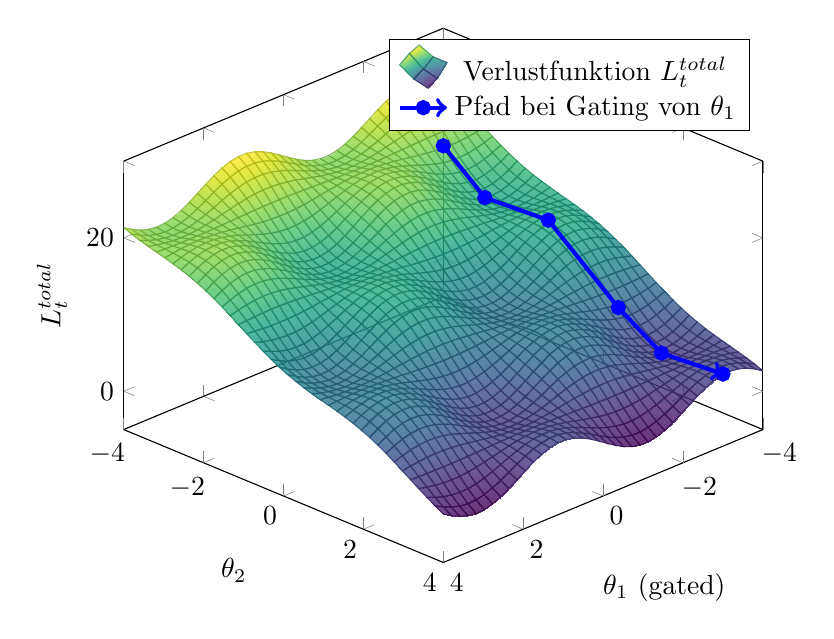
\begin{tikzpicture}
        \begin{axis}[
            width=0.8\textwidth,
            view={135}{35}, % Blickwinkel angepasst für Diagonale
            xlabel=$\theta_1$ (gated),
            ylabel=$\theta_2$,
            zlabel=$L_t^{total}$,
            colormap/viridis,
            zmin=-5, zmax=30, % Angepasste Z-Grenzen
        ]
        
        % 1. Die Oberfläche (identisch zur ersten Grafik)
        \addplot3[
            surf,
            shader=faceted interp,
            domain=-4:4,
            y domain=-4:4,
            samples=40,
            opacity=0.8
        ] {12 - 2.5*y + 2.5*sin(deg(x*1.5))*cos(deg(y*1.5))};

        % 2. Der Pfad des Gradientenabstiegs mit Gating
        % Theta_1 ist fixiert bei -3, der Pfad bewegt sich nur entlang Theta_2
        \addplot3[
            color=blue,
            mark=*,
            mark size=2pt,
            line width=1.5pt,
            ->
        ] coordinates {
            (-3, -3, 19.0)    % Start
            (-3, -1.96, 14.5) % Abstieg nur in y
            (-3, -0.37, 15.0)
            (-3, 1.38, 7.4)
            (-3, 2.46, 3.8)
            (-3, 4.0, 4.4)    % Ende
        };
        
        \legend{Verlustfunktion $L_t^{total}$, Pfad bei Gating von $\theta_1$}
        \end{axis}
    \end{tikzpicture}
    \caption{Auswirkung von Gradient Gating auf den Optimierungspfad. Da der Parameter $\theta_1$ vom Rückfluss der Gradienten ausgeschlossen ist, erfolgt die Optimierung ausschließlich entlang der Achse $\theta_2$. Der Parameter $\theta_1$ verharrt auf seinem Initialwert.}
    \label{fig:gradient_descent_gated}
\end{figure}
\vspace{\baselineskip}

Es ist wichtig anzumerken, dass diese Visualisierung eine Projektion des hochdimensionalen Parameterraums auf zwei Dimensionen darstellt. $\theta_1$ steht hierbei stellvertretend für alle Netzwerk\hyp{}Gewichte, die einem aktuell inaktiven Aktionszweig zugeordnet sind, während $\theta_2$ die Parameter des aktiven Zweigs repräsentiert. In der Praxis führt das Gating dazu, dass die Parameter des inaktiven Zweigs ($\theta_1$) eingefroren werden und somit vor dem Einfluss von Rauschen geschützt sind, solange ihre Aktion nicht zur Ausführung kommt.

\section{Metriken im Reinforcement Learning}
Um den Erfolg der durchgeführten Experimente und die Wirksamkeit der modifizierten Algorithmen in Kapitel \ref{ch:evaluation} quantitativ bewerten zu können, müssen geeignete Vergleichsgrößen definiert werden. Im Reinforcement Learning gibt es verschiedene Metriken, die verwendet werden, um die Leistung eines Agenten zu bewerten.
Diese Metriken helfen dabei, den Fortschritt des Lernprozesses zu überwachen und die Effektivität verschiedener Algorithmen und Hyperparameter zu vergleichen.
Viele dieser Metriken werden automatisch von \ac{RL}\hyp{}Bibliotheken wie Stable Baselines3 \cite{sb3} erfasst und können zur Analyse und Visualisierung verwendet werden.
Dieser Abschnitt soll sich auf diese \ac{PPO}\hyp{}spezifischen Metriken konzentrieren. Die Umgebungs\hyp{}spezifischen Metriken werden im Abschnitt \ref{sc:env_metrics} beschrieben.
Folgende Metriken sind besonders relevant \cite{LogExplanation}:
\begin{itemize}
    \item \textbf{Explained Variance (EV):} Diese Metrik misst, wie gut der Critic die tatsächlichen Returns vorhersagt. Ein hoher EV\hyp{}Wert (nahe 1) deutet darauf hin, dass der Critic
    die Returns gut modelliert, während ein niedriger oder negativer Wert auf eine schlechte Vorhersage hinweist.
    \item \textbf{Policy Loss:} Dies ist der Verlust, der bei der Aktualisierung der Policy berechnet wird. Ein negativer Wert ist wünschenswert, da der Loss minimiert werden soll. 
    Ein stark positiver Wert kann auf Instabilitäten im Lernprozess hinweisen.
    \item \textbf{Value Loss:} Dies ist der Verlust, der bei der Aktualisierung des Critic\hyp{}Netzwerks berechnet wird. Ein negativer Wert ist wünschenswert, da der Loss minimiert werden soll. 
    Ein stark positiver Wert kann auf Instabilitäten im Lernprozess hinweisen.
    \item \textbf{Entropy Loss:} Diese Metrik quantifiziert die Entropie (Zufälligkeit) der Aktionsverteilung des Agenten. Sie dient als Maß für die Exploration: 
    Eine hohe Entropie bedeutet eine breite Streuung der Aktionen und fördert das Entdecken neuer Strategien, während eine sinkende Entropie auf eine zunehmende 
    Spezialisierung (Exploitation) der gelernten Policy hindeutet. In der Optimierungslogik wird die Entropie mit einem negativen Vorzeichen versehen, um sie 
    als Minimierungsproblem darzustellen. Da der Algorithmus den Gesamt\hyp{}Loss minimiert, führt ein negativer Entropy Loss effektiv zu einer Maximierung der Entropie. 
    Ein Wert, der gegen Null strebt, signalisiert somit, dass der Agent eine deterministische Strategie entwickelt hat und die Exploration abgeschlossen ist.
    \item \textbf{Clip Fraction:} Diese Metrik gibt an, wie oft das Wahrscheinlichkeitsverhältnis \(r_t(\theta)\) im Clipped Surrogate Objective beschnitten wurde.
    Ein hoher Clip Fraction\hyp{}Wert kann darauf hinweisen, dass die Policy\hyp{}Updates zu aggressiv sind, was die Stabilität des Lernprozesses beeinträchtigen kann.
    \item \textbf{Approx KL:} Diese Metrik approximiert die Kullback\hyp{}Leibler\hyp{}Divergenz zwischen der alten und neuen Policy. Sie dient als Maß für die Änderung 
    der Policy während des Lernprozesses. Ein hoher Approx KL\hyp{}Wert deutet auf eine signifikante Policy\hyp{}Änderung hin, was auf eine aggressive Aktualisierung hindeutet.
\end{itemize}

Diese Metriken bieten wertvolle Einblicke in den Lernprozess und helfen dabei, die Leistung des \ac{RL}\hyp{}Agenten zu bewerten und zu optimieren.
Metriken wie Explained Variance, Policy Loss, Value Loss und Entropy Loss sind entscheidend, um den Trainingsfortschritt zu überwachen und sicherzustellen, dass der Agent effektiv lernt. Approx KL und Clip Fraction geben zusätzlich Hinweise auf die Stabilität der Policy\hyp{}Updates. Sprünge oder ungewöhnliche Muster in diesen Metriken können auf Probleme im Lernprozess hinweisen, die eine Anpassung der Hyperparameter oder der Algorithmus\hyp{}Architektur erfordern.




